\documentclass[a4paper,11pt] {article}
\usepackage{graphicx}
\usepackage{amssymb, amsmath, amsthm}
\usepackage{setspace}
\usepackage{amsfonts}

%-----------Margin, Linespread, Spacing-----------%
\usepackage[letterpaper, margin=1.3in]{geometry}
\usepackage[letterpaper]{geometry}
\linespread{1}
%-------------------------------------------------%

%-----------Define header and footnotes-----------
\usepackage{fancyhdr}               % Header and footnotes
\pagestyle{fancy}
\lhead{\bfseries \scriptsize CQF}
\chead{\bfseries \scriptsize Module 5 Solution}
\rhead{\bfseries \scriptsize Ran Zhao}
\renewcommand{\headrulewidth}{0.4pt}
%-------------------------------------------------%

%---------------------Listings--------------------%
\usepackage{listings}
\usepackage{color}
\definecolor{dkgreen}{rgb}{0,0.6,0}
\definecolor{gray}{rgb}{0.5,0.5,0.5}
\definecolor{mauve}{rgb}{0.58,0,0.82}
\lstset{ %
  language=Octave,                % the language of the code
  basicstyle=\footnotesize,           % the size of the fonts that are used for the code
  numbers=left,                   % where to put the line-numbers
  numberstyle=\tiny\color{gray},  % the style that is used for the line-numbers
  stepnumber=2,                   % the step between two line-numbers. If it's 1, each line
                                  % will be numbered
  numbersep=5pt,                  % how far the line-numbers are from the code
  backgroundcolor=\color{white},      % choose the background color. You must add \usepackage{color}
  showspaces=false,               % show spaces adding particular underscores
  showstringspaces=false,         % underline spaces within strings
  showtabs=false,                 % show tabs within strings adding particular underscores
  frame=single,                   % adds a frame around the code
  rulecolor=\color{black},        % if not set, the frame-color may be changed on line-breaks within not-black text (e.g. commens (green here))
  tabsize=2,                      % sets default tabsize to 2 spaces
  captionpos=b,                   % sets the caption-position to bottom
  breaklines=true,                % sets automatic line breaking
  breakatwhitespace=false,        % sets if automatic breaks should only happen at whitespace
  title=\lstname,                   % show the filename of files included with \lstinputlisting;
                                  % also try caption instead of title
  keywordstyle=\color{blue},          % keyword style
  commentstyle=\color{dkgreen},       % comment style
  stringstyle=\color{mauve},         % string literal style
  escapeinside={\%*}{*)},            % if you want to add LaTeX within your code
  morekeywords={*,...}               % if you want to add more keywords to the set
}
%-------------------------------------------------%

%----------------Title, Author, Dates-------------
\author{Ran Zhao}
\title{CQF Module 5 Exercise Solution}
\date{}
\begin{document}
\maketitle
%--------------------------------------------------


\textcolor{blue}{\bf 1 a} To compute the firm's asset value and volatility, set up the Merton type structural model as
\begin{eqnarray*}
E_0 &=& V_0  N(d_1) - D \exp (-rT) N(d_2) \\
d_1 &=& \frac{1}{\sigma_V} \left[ \log \left(\frac{V_0}{D} \right) + \left( r + \frac{1}{2}\sigma_V^2 \right) T \right] \\
d_2 &=& d_1 - \sigma_V \sqrt{T} \\
\sigma_E &=& \sigma_V N(d_1) \frac{V_0}{E_0}
\end{eqnarray*}

To solve the simultaneous equations numerically, I use MATLAB to find the minimum of the penalty function, where the deviations of $E_0$ and $\sigma_E$ between what are given in the context and computed results are calculated. The optimization results yield

$$ \left\{
\begin{aligned}
V_0 &=& 7.9088 \\
\sigma_V &=& 19.12\%
\end{aligned}
\right.
$$

Substitute the solutions into the simultaneous equations above, we yield back the equity value and equity volatility. The codes solving the equations are provided in the Appendix.

\bigskip

\textcolor{blue}{\bf 1 b} The probability of the default for Merton model is
$$
\mathbb{P}[V_t < D] = N(-d_2)
$$
whereas in the Black-Cox PD is calculated as
$$
\mathbb{P}[\tau \leq T | \tau > t] = N(h_1) + \exp\left\{ 2\left(r-\frac{\sigma_V^2}{2}\right) \log\left( \frac{K}{V_0} \right) \frac{1}{\sigma_V^2} \right\} N(h_2)
$$

Using the simultaneous equations in (1a) to solve for $V_0$ and $\sigma_V$, we have the following sensitivity between $\sigma_E$ and the probability of default.

\begin{center}
\begin{figure}
  \centering
  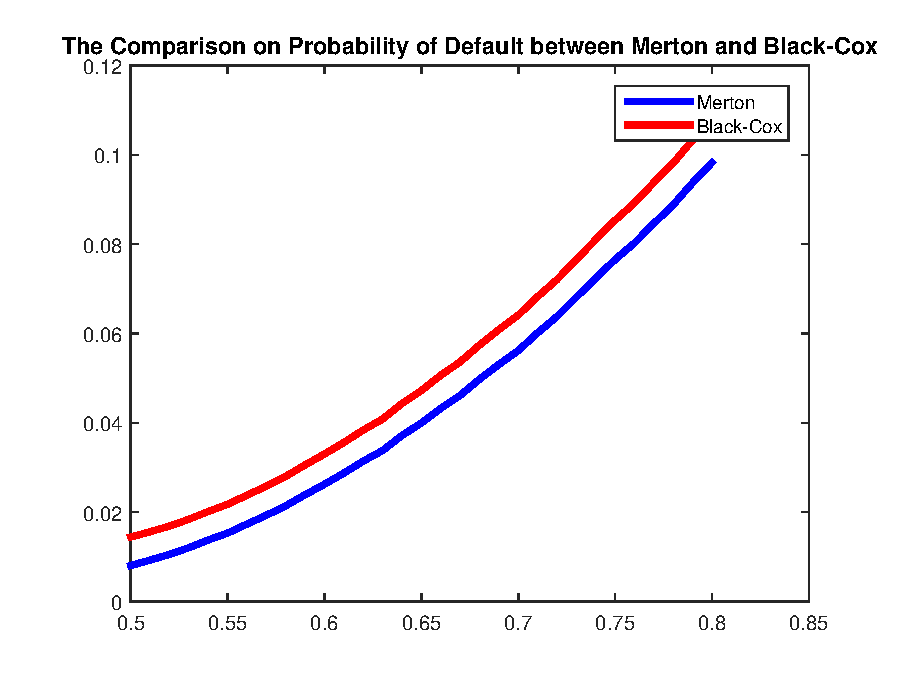
\includegraphics[scale=0.7]{PDs.eps}
  \caption{The comparison of probability of default between Merton and Black-Cox Models}\label{fig::PDs}
\end{figure}
\end{center}

As shown in Figure~\ref{fig::PDs}, the probability of default increases with higher equity volatility. Intuitively speaking, the higher equity volatility makes it more possible for asset value to fall below the debt, and therefore more like to default. 

The Merton model estimates PD lower than the Black-Cox model, for the reason that the Black-Cox allows for early default than the maturity. Beyond equity volatility as 60\%, the probability of default increases monotonically with the equity volatility, and the PD estimated by Black-Cox model is 0.8\%.

The codes solving the equations are provided in the Appendix.

\bigskip

\textcolor{blue}{\bf 2 a}


\section*{Appendix}
\begin{spacing}{0.9}
\lstinputlisting[language=Matlab]{compute_E0.m}
\lstinputlisting[language=Matlab]{compute_value_vol_1a.m}
\end{spacing}

\end{document} 